\begin{tikzpicture}[remember picture,overlay]
  \node[
    draw,
    minimum width=18cm,
    minimum height=1cm,
    text width=17cm,   % texten får en paragrafyta att "jobba i"
    align=left,        % vänsterjustera texten
    anchor=west        % så att (7,1) är vänsterkanten av boxen
  ] at (-1.5,1)
  {Title: Project Plan};

  \node[
    draw,
    minimum width=5cm,
    minimum height=1cm,
    text width=6cm, 
    align=left,
    anchor=west   
  ] at (10.3,1) {ID: PP-01\\ 
  Version: 1.0};

    % Nedre vänstra rektangeln
  \node[
    draw,
    minimum width=6cm,
    minimum height=1cm,
    text width=5.5cm,
    align=left,
    anchor=west
  ] at (-1.5,0)
  {Author:\\ Andrea Haglund};

  % Nedre mitten rektangeln
  \node[
    draw,
    minimum width=5.8cm,
    minimum height=1cm,
    text width=5.5cm,
    align=left,
    anchor=west
  ] at (4.5,0)
  {Role: \\ Chief Engineer};

  % Nedre högra rektangeln
  \node[
    draw,
    minimum width=6cm,
    minimum height=1cm,
    text width=6cm,
    align=left,
    anchor=west
  ] at (10.3,0)
  {Page 1 of 29.};
  
\end{tikzpicture}

\vspace{3 cm}

\begin{center}
    \LARGE\textbf{DOCUMENT APPROVAL}\\
    
    \vspace{0.5 cm}
    
    \begin{tabular}{|l|l|l|l|l|}
        \hline
        Name & Role & Version & Date & Signature \\
        \hline
             &      &         &      &           \\
        \hline
     \end{tabular}
     
     \vspace{3 cm}
     
     \LARGE\textbf{DOCUMENT CHANGE RECORD}\\
     
     \vspace{0.5 cm}
     
     \begin{tabular}{|l|l|l|l|l|}
        \hline
        Version & Date & Reason for Change & \makecell{Pages/Sections\\ Affected} \\ \hline
        0.1 & 2025-09-29 & Version for internal review &  \\ 
        \hline
        0.2 & 2025-10-01 & Version for review &  \\ 
        \hline
        1.0 & 2025-10-02 & \makecell{Version for public release} &  All \\ 
        \hline
   \end{tabular}
\end{center}